\documentclass[12pd]{article}
\usepackage[utf8]{inputenc}
\usepackage[T2A]{fontenc}
\usepackage[mongolian]{babel}
\usepackage{graphicx}
\graphicspath{ {images/} }
\title{Журнал}
\author{Б. Баясгалан B140920586}


\begin{document}
	
	\section {Оршил}
	\subsection {Төслийн ажлын зорилго}
	\begin{itemize}
		\item Системийн хэрэглэгчидийн  хоорондын  харилцаа үйл ажилгаа   хялбар албадаагүй тодорхой болгож цаг хугацааг хэмнэх  зорилготой. Дүнгийн мэдээлэл, хичээлийн хуваарь  гэх зэрэг мэдээллийг хүссэн   байрлалаасаа хандаж  нэг доор  хурдан шуурхай өгөх
	\end{itemize} 
	\subsection { Төслийн ажлын зорилт}
	\begin{itemize}
		\item Системийн хяналт ,шалгалтыг  сайжруулж  бодитой дүн гаргах
		\item Зардал, цаг хугацаа хэмнэлт хийх  
		\item Мэдээллийн аюулгүй байдал, нууцлал болгох
	\end{itemize}
\subsection {Системийн хүрээ  хязгаар}
\begin{itemize}
	\item ШУТИС-МХТ сургуулийн  багш , сурагчид эцэг эхчүүд   ашиглах боломжтой
\end{itemize}
\section{Судалгаа}
\subsection{Програмын судалгаа}
\subsubsection{Монголын  системүүдийн харьцуулсан судалгаа}

\begin{itemize}
	\item  Улирлын жилийн эцсийн дүн хичээлийн явцыг удирдах сурагч болон эцэг эхчүүдийн системд нэвтрэх эрхийг үүсгэх боломжтой.Удирдсан ангийн сурагчдын мэдээлэлтэй ажиллах, ангийн хичээлийн хуваарь, ирцийн мэдээлэл, сургалтын мэдээлэл, ангийн журнал харах, тайлан гаргах, ангийн сурагчийн жилийн эцсийн тодорхойлолт, ангийн дүнгийн хавтгай гаргах боломжтой. Мөн өөрийн сургалтын мэдээлэл харах, өөрийн ирцийн мэдээлэлтэй танилцах, өөрийн хичээлийн хуваарь харах, заасан хичээлийн тэмдэглэл хөтлөх, заадаг ангийн сурагчдийн дүн, ирцийн мэдээлэл оруулах, ерөнхий тайлан гаргах зэрэг үйлдлүүдийг хийж блно.лирлын жилийн эцсийн дүн хичээлийн явцыг удирдах сурагч болон эцэг эхчүүдийн системд нэвтрэх эрхийг үүсгэх боломжтой.
	\item Эцэг эхчүүд нь  багш, сургууль байнгын холбоо харилцаатай байх боломжтой  бөгөөд хүүхдийнхээ хичээлд оролцсон байдал ирц, хичээлийн хуваарь, болон бусад мэдээллүүдтэй танилцах, заасан хичээлүүдийн хөтөлбөрийг нь харах боломжтой юм.
	
	\subsubsection{ТЭЭВРИЙН ДЭЭД СУРГУУЛЬ оюутны веб (
		)}
	\item Эцэг эхчүүд  хүүхдийнхээ  хичээлийн оролцоо дүнг мэдээлэл авах,хянах боломжтой
	\item Сурагч хичээлийн хуваарь, дүнгийн мэдээлэл  явцын дүн мэдэх боломжтой

	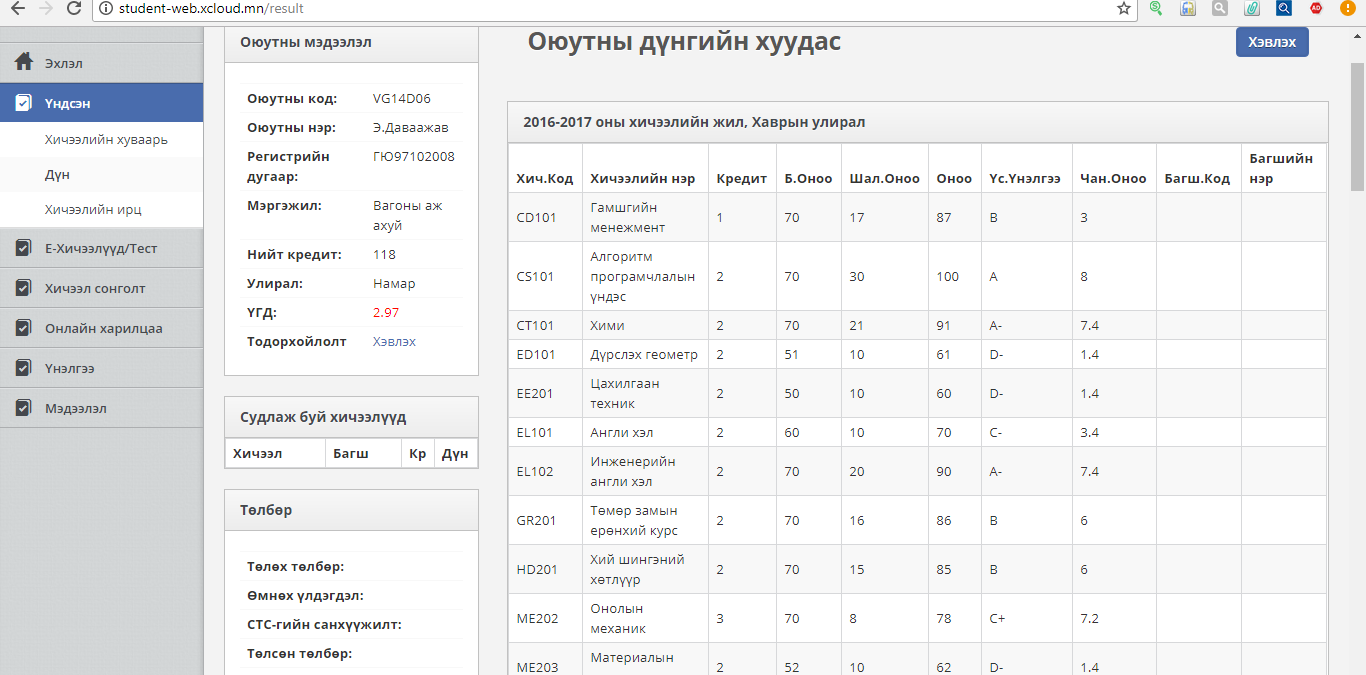
\includegraphics[width=\textwidth]{zurag}
\end{itemize}

	\section {Системийн шаардлага}

	\subsection { Програмын хэрэглэгчид }
	\begin{itemize}
		\item Багш
		\item Сурагч 
		\item Эцэг эх
	\end{itemize}
	\subsection {Функциональ шаардлага}
		\begin{itemize}
		\item Багш дүгнэх журам оруулах
		\item Сурагчдийн ирц оруулах
		\item Сурагчдийн явцын оноо оруулах 
		\item Сурагчын мэдээллийг кодоор хайх
		\item Сурагчын дэлгэрэнгүй мэдээллийг харах
		\item Багш өөрийн зааж байгаа хичээлийн сурагч нарыг харах
		\item Сурагч дүгнэх журам харах
		\item Сурагч ирц харах
		\item Сурагч явцын оноо харах
		\item Эцэг эх хүүхэдийнхээ дүнгийн мэдээлэлийг харах
		\item Эцэг эх хүүхэдийнхээ ирцыг харах
		\item Эцэг эх хүүхэдийнхээ явцыг харах
	\end{itemize}
	
	\subsection{ Функциональ бус шаардлага}
	\begin{itemize}
		\item Сургалтын хэлбэрт зохицсон байх
		\item Хэрэглэхэд хялбар ойлгомжтой, дэлгэрэнгүй байх
		\item Мэдээллийг түргэн шуурхай харуулдаг байх
	\end{itemize}
	
	\section {Юзкейс диаграм}
	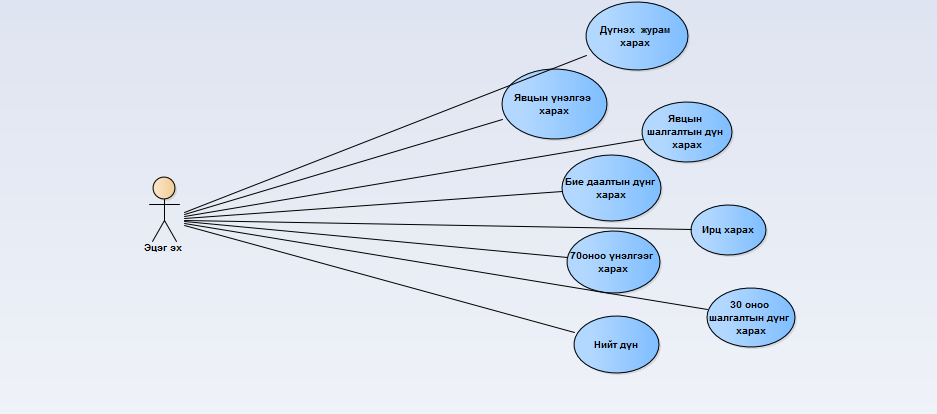
\includegraphics[width=\textwidth]{Usecase1}
	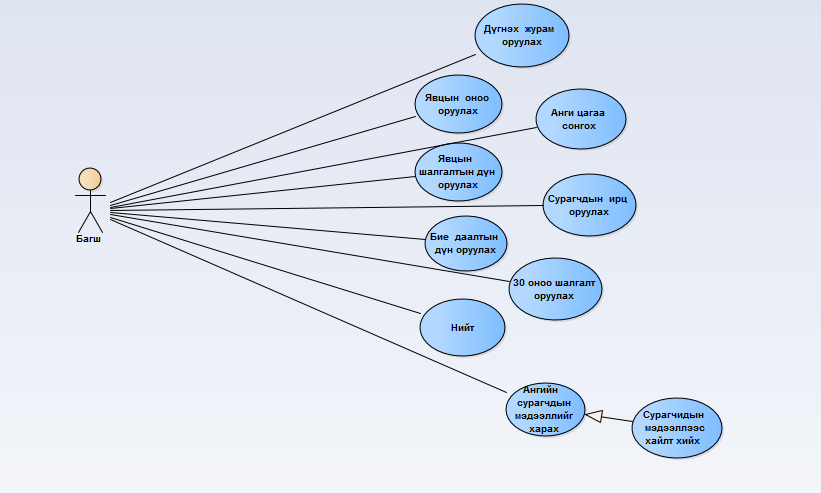
\includegraphics[width=\textwidth]{Usecase2}
	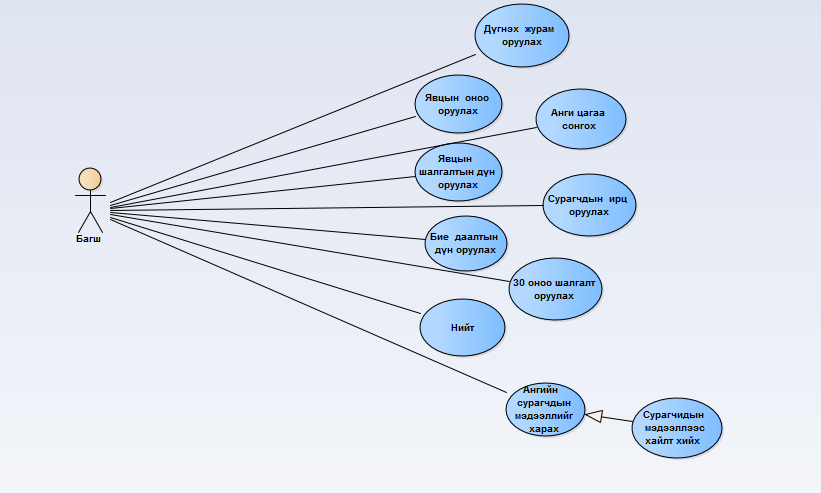
\includegraphics[width=\textwidth]{Usecase3}
	\section{Дэлгэц}
	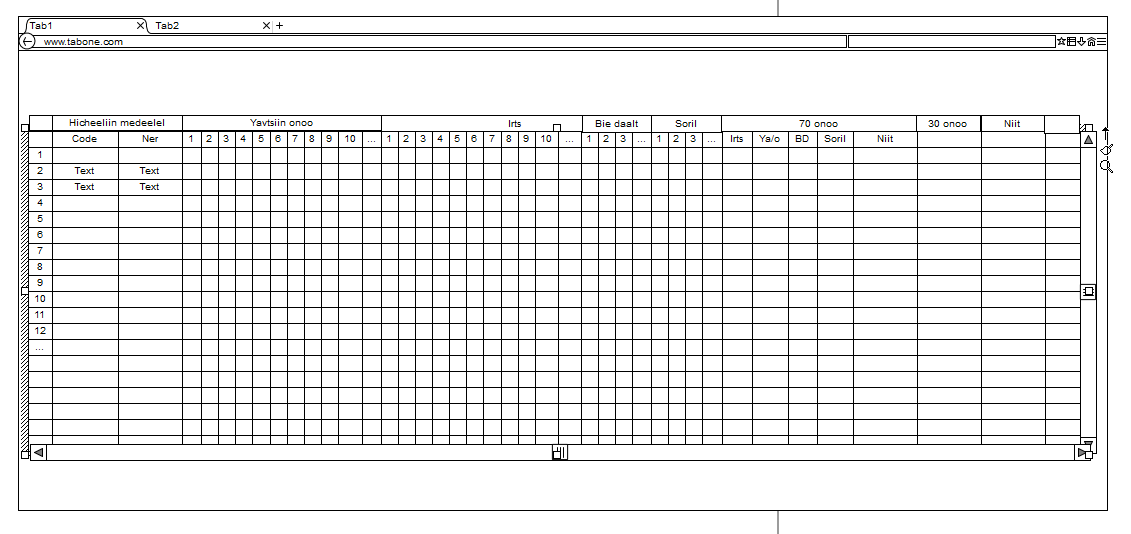
\includegraphics[width=\textwidth]{delgets}
	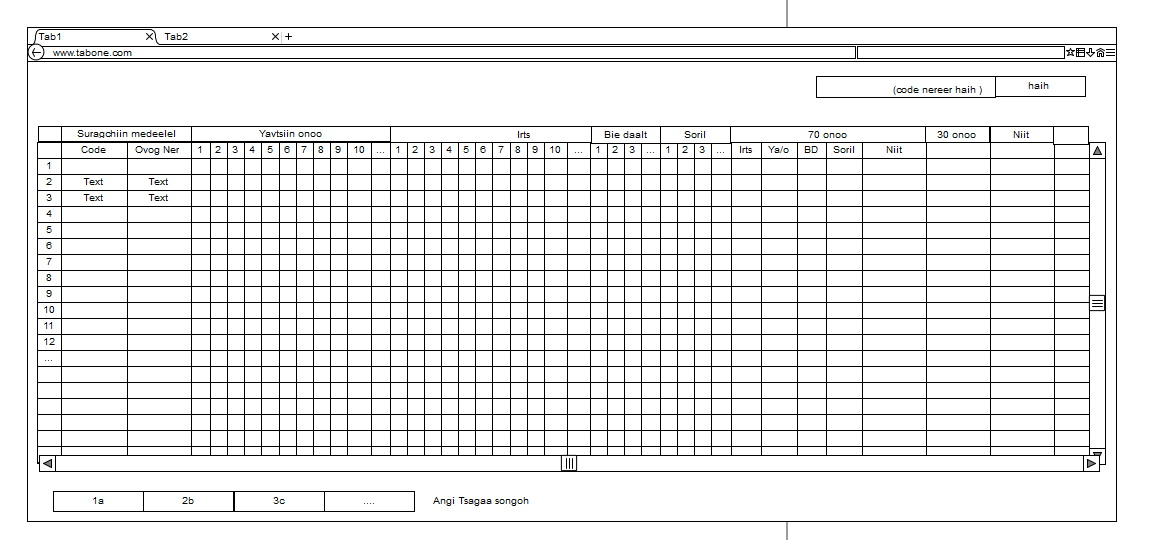
\includegraphics[width=\textwidth]{delgets2}
	\section{Үйл ажиллагааны диаграм (Activity diagram)}
	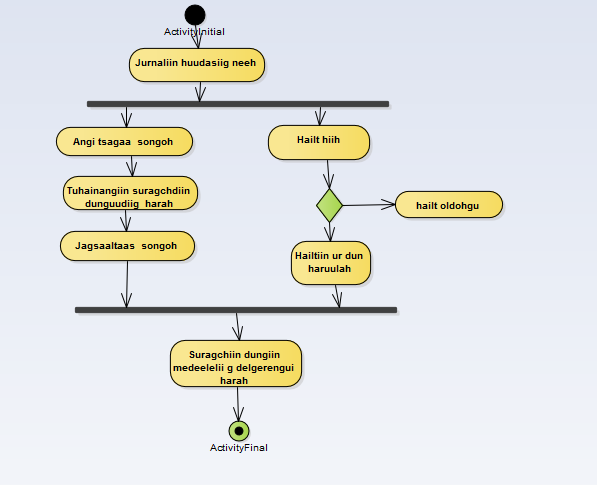
\includegraphics[width=\textwidth]{ac1}
	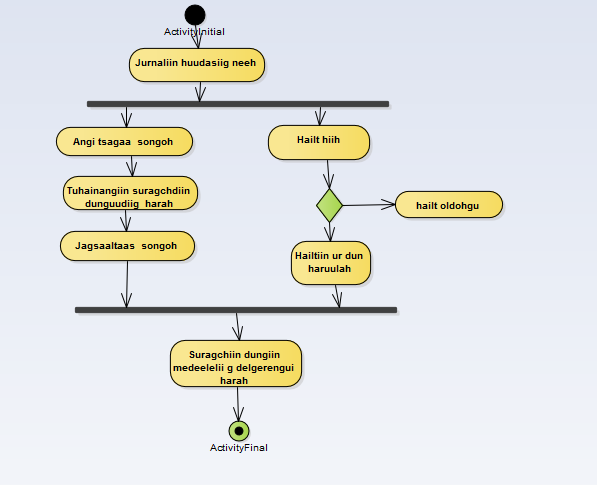
\includegraphics[width=\textwidth]{ac2}
	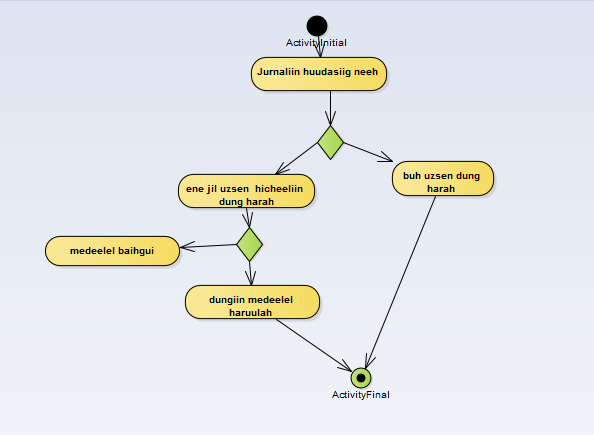
\includegraphics[width=\textwidth]{ac3}
	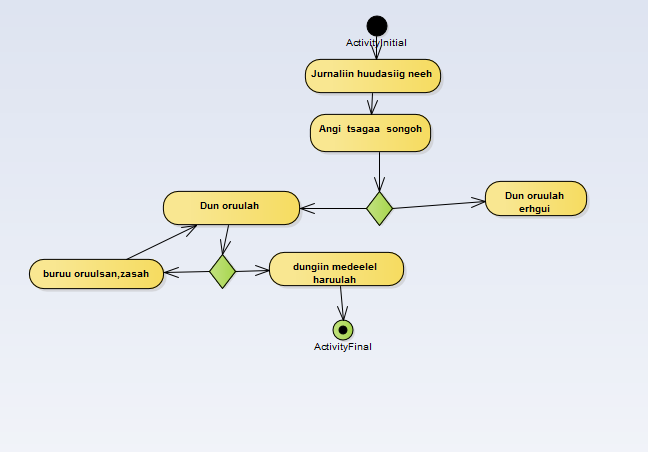
\includegraphics[width=\textwidth]{ac4}
	\section{Обьедтийн  холбоосын  диаграм (ERD)}
	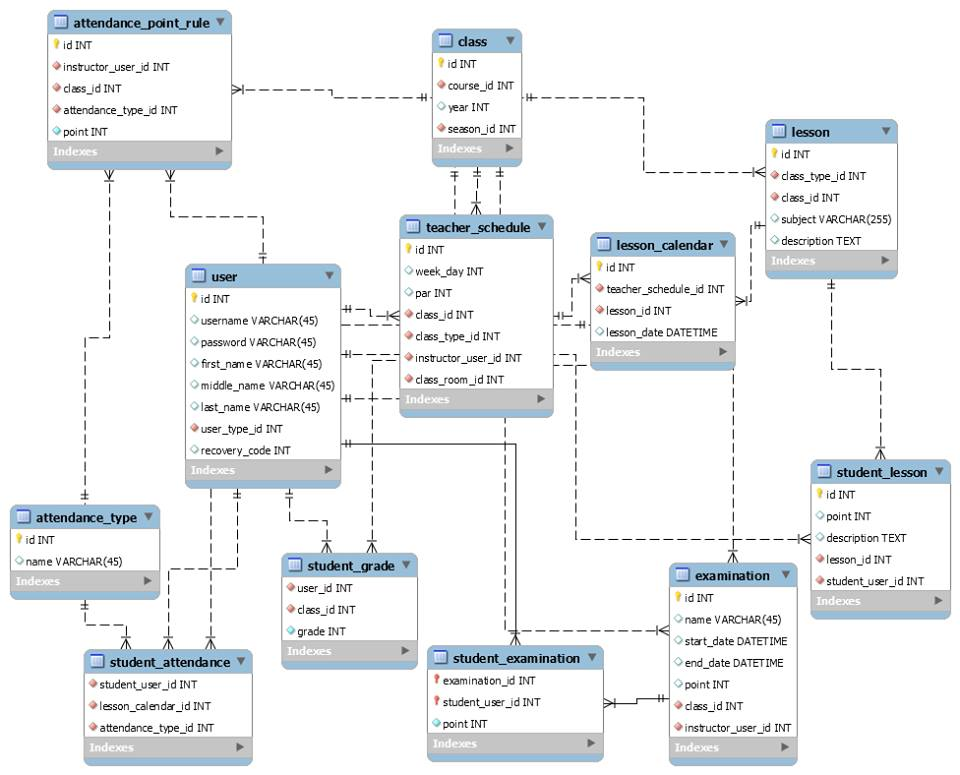
\includegraphics[width=\textwidth]{jurnal}
	\section {Класс  диаграм (Class diagram )}
		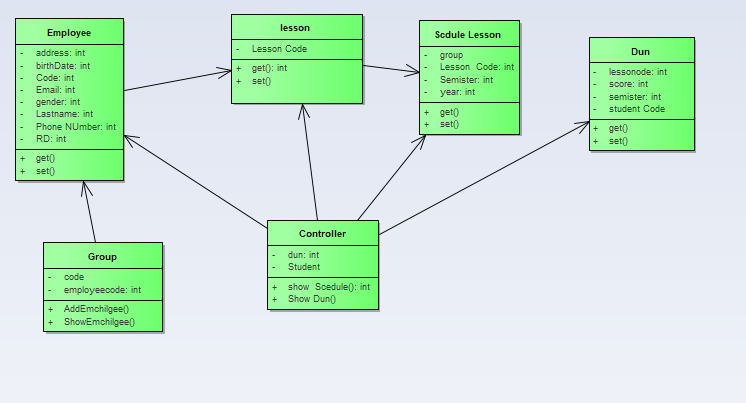
\includegraphics[width=\textheight]{clss}
	\section{Дарааллын  диаграм(Sequence diagram)}
	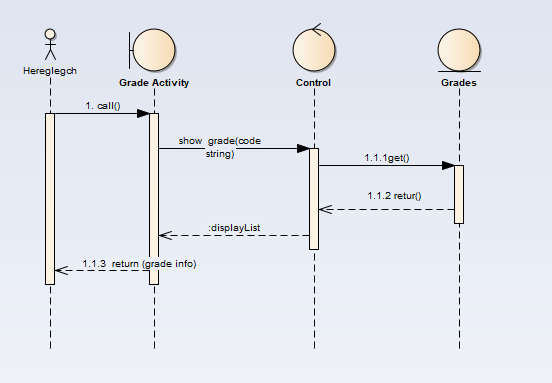
\includegraphics[width=\textheight]{se1}
	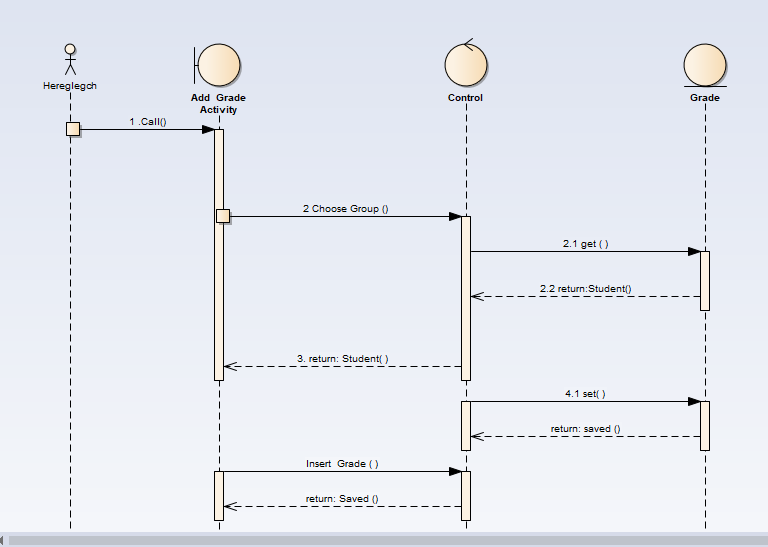
\includegraphics[width=\textheight]{se2}
\section {Дүгнэлт}
\begin{itemize}
	\item 
	\end{itemize}

	
					
				
\end{document}